% ===================================================================================================
%                                                 |                                                 |
%                                                 |                                                 |
% -------------------------------------------- SECTION ---------------------------------------------|
%                                                 |                                                 |
%                                                 |                                                 |
% ===================================================================================================
\section{Introduction}\label{sec:intro}
%---
\begin{fancyquotes}
	AI is one of the cornerstones of the growing digitization of industry ('Industry 4.0'). Technologies underpinning  this  process  ---  such as IoT,  5G,  \textbf{cloud  computing},  big  data  analytics,  \textbf{smart  sensors},  augmented  reality,  3D  printing  and  \textbf{robotics}  ---  are  likely  to  transform  manufacturing  into  a  single cyber-physical  system  in which digital  technology,  internet  and  production  are merged in one \cite{szczepanski_2019}.
\end{fancyquotes}
%---
As Industry 4.0 continues to develop, smart factories will become the norm. They will be populated with modern industrial, collaborative and service robots with local and network computing capabilities collecting and sharing data from their myriad of sensors. %, see Fig~\ref{fig:smartFactory}.
AI will be a natural component of these robots, enabling them to learn new tasks and spread their knowledge across systems. The more these robots are synergistically integrated into manufacturing, they will independently take care of diverse tasks and also collaborate with humans. Yet, as embodied AI agents become ubiquitous, new challenges will emerge, among them, their energy demand.

% SUBSECTION ========================================================================================
\subsection{The energy problem in classical and embodied AI}
%---
% \begin{figure}[!t]
% 	\centering
% 	\includegraphics[width=0.99\columnwidth]{fig/smart_factory.pdf}
% 	\caption{The smart factory.}
% 	\label{fig:smartFactory}
% \end{figure}

Classical AI interprets intelligence as a purely computational symbol processing problem decoupled from corporeal agents. Progress in classical AI relies on two computing stages: (1) learning and (2) deployment. While the latter is certainly not energy-efficient compared to its biological counterparts, the former craves a large energy quota, used to process large amounts of data for training, validation and testing of models (e.g. super computing). Furthermore, it is expected that both, model and training data, carry enough information to allow knowledge transfer between different tasks and even systems (at least to a certain extent). However, retraining is required when this information is not available in the data, sometimes even from scratch, leading to highly energy inefficient learning paradigms. This implies that the energetic cost of classical AI sometimes outweighs its benefits \cite{Strubell2019EnergyAP}. Furthermore, with the coming evolution towards \emph{embodied AI} systems, i.e. the emerging field between AI and robotics, the challenges mentioned before expand. Since the real world cannot be simply captured as a form of database, \textcolor{red}{despite various works claiming otherwise \textbf{[REF]}}, data acquisition in embodied AI agents necessitates from constant and active energy-expending interaction with the physical environment. Likewise, learning a task implies physically executing it, and with each execution energy is required for motion and interaction. Take for example autonomous driving, where the vehicle is a rather basic form of an embodied AI agent. Despite operating mostly in a structured man-made environment, complexity is already present in the system as the vehicle spends energy simply by carrying out its purpose: autonomous movement; but also spends energy by collecting vast amounts of data (obtained by driving around) to then retrain and improve the policy model in real-time. \textcolor{red}{Additionally, the energy to build the offline model has to be taken into consideration.} While in the last years the energy demand of AI and robotics entered the scope of separate research communities, we argue and substantiate that the study of the energetic requirements of embodied AI and its vast implications has not received proper attention. 
% ---
\begin{figure*}[!t]
	\centering
	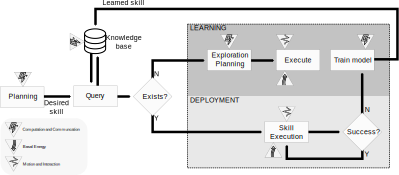
\includegraphics[width=0.9\textwidth]{fig/embodied_ai_learning_pipeline_v7.pdf}
	\caption{Standard task execution pipeline in isolated embodied AI systems.}
	\label{fig:embodied_ai_pipeline}
\end{figure*}
% ---
% SUBSECTION ========================================================================================
\subsection{Contributions}
To facilitate the study of the energetic demand of embodied AI systems, we look at the standard task execution pipeline in an isolated embodied AI agent, shown in Fig.~\ref{fig:embodied_ai_pipeline}, and identify three main categories of energy usage, namely 
\begin{enumerate}
    \item Computation and Communication Expenditure (CCE): refers to the energy required by the computation process itself (e.g. the number of floating point operations) and by the supporting communication processes
    \item Basal Energy Expenditure (BEE): this is the energy associated to the basic functions of the robot. For example gravity compensation and proprioceptive intelligence/algorithms in robots, hovering in drones, collision avoidance in autonomous vehicles, etc.
    \item Motion and Interaction Expenditure (MIE): defines the energy spent on executing a particular task in a given way
\end{enumerate}
 \textcolor{red}{To form a complete on the energy balance, the energy usage in the manufacturing, recycling and disposal of embodied AI agents should also be considered; however, it is outside the scope of this work. We will center our attention to, in particular, the learning and deployment routines.} We provide projections on the growing energetic challenges in embodied AI pertaining to these categories and show that the energy demand scales out of proportion if the current isolated learning paradigms are further maintained. Furthermore, we establish that with the scaling complexity of the problems faced by classical and embodied AI, clever learning methods are required, that make not only efficient use of the computation and physical power of the embodied agent but also leverage modern communication infrastructure to optimally collect, share, and transfer the knowledge acquired by other agents performing similar tasks. We then show that isolated learning proves to be insufficient to find an energy-minimizing solution and that also incremental and even transfer learning are still incomplete strategies to maximally reduce energy demand to a sustainable level. In consequence, we prove collective learning as the most general and capable learning paradigm that can globally minimize the energy consumption in embodied AI systems. For this, we contextualize the problem in a hypothetical case study  making use of empirical/reported estimations of energy consumption and introducing a full energy estimation model that accounts for the three energy expenditure categories (CCE, BEE and MIE). Concretely, we estimate the substantial effect that collective learning can have on energy and time saving {\color{red}{in a smart factory scenario with a large number of robots performing a large number of tasks probably existing in the near future}}. With this we show that collective learning is the natural solution to address the energy problem in embodied AI and leads to more tasks learnt in shorter time needing less energy.

% SUBSECTION ========================================================================================
\subsection{Paper organization}
\TODO